\section{Strukturanalyse} \label{kap:3}
\begin{itemize}
    \item[(a)] Direkte Abbildung:\\
          \begin{itemize}
              \item Transmissions-Elektronen-Mikroskopie (TEM)
              \item Raster-Tunnel-Mikroskopie (STM)
          \end{itemize}
          Atomare Auflösung, aber nur oberflächenintensiv
    \item[(b)] \textbf{Beugungs-/ Streuexperimente:}\\
          Grundidee:
          \begin{itemize}
              \item Einstrahlung einer Welle (elektromagnetische Welle, Materiewelle) auf den periodischen Festkörper (Gitterkonstante $a \approx$ 1 \AA)\\
                    Bedingung für Beugung: $\lambda < \approx a$\\
                    z.B. Röntgenstrahlung mit $\lambda \approx$ 1 \AA ($h \nu$ = 12 keV)\\
                    Elektronen mit $\lambda \approx$ 1 \AA ($h \nu$ = 150 eV)\\
                    Neutronen mit $\lambda \approx$ 1 \AA ($h \nu$ = 80 meV)\\
                    He-Atome mit $\lambda \approx$ 1 \AA ($h \nu$ = 20 meV)
              \item Je nach Art der Welle unterschiedliche Eindringtiefe Röntegen- u. Neutronensteuung $\rightarrow$ massive FK, Elektronen - u. Atomstreuung eher für dünne Filme / Oberflächen.
              \item Je nach Art der Welle Information über Elektronen- bzw. Kernverteilung. Beugungsmuster bei bekannten $\lambda$ liefert Informationen über periodische Anordnung des Kristalls.\\
                    Man unterscheidet
                    \begin{itemize}
                        \item \textbf{Kohärente Streuung} (Information über Struktur) oder inkohärente Streuung
                        \item \textbf{Elastische Streuung} (Strukturbestimmung) oder inelastische Streuung (Untersuchung von elektronischen oder vibronischen Anregungen)
                    \end{itemize}
          \end{itemize}
\end{itemize}





\subsection{Einführung in die Streutheorie} \label{kap:3_1}
Grundannahmen: Klassische Beschreibung der Streuung, elastische Streuung, Einfachstreuung
\begin{itemize}
    \item Einlaufende Welle und auslaufende Welle sind eben Wellen (Guta Annahme, falls Quelle bzw. Beobachter weit entfernt)
          \begin{figure}[H]
              \centering
              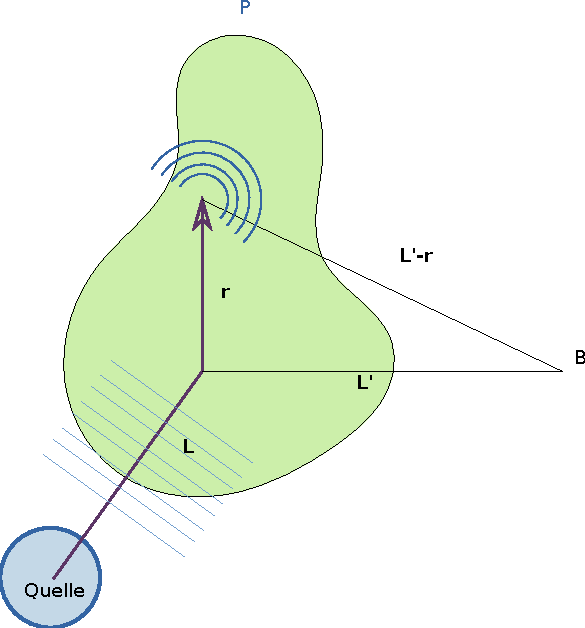
\includegraphics{figures/2_4Birne.pdf}
              \caption{}
              \label{}
          \end{figure}
    \item Einlaufende welle mit Amplitude $A_P = A_0 e^{-i(\omega_0 t - \textbf{k} ( \textbf{L} + \textbf{r}))}$
    \item Auftreffen auf Verteilung von Streuzentren mit komplexwertiger Streudichteverteilung $\rho(\textbf{r})$, die vom Ort und von Art der WW abhängt.
    \item Jedes Streuzentrum (z.B. P) emittiert eine Kugelwelle, deren Amplitude und Phase relativ zur einlaufenden Welle con $\rho(\textbf{L} + \textbf{r})$ abhängt.
          \begin{align*}
              A_B^P                   & = A_P \cdot \rho(\textbf{L} + \textbf{r}) \frac{e^{i\textbf{k}' ( \textbf{L}' - \textbf{r})}}{|\textbf{L}' - \textbf{r}|}                                                                   \\
                                      & \approx \frac{A_0}{L'} e^{-i \omega_0 t} e^{i \textbf{k} \textbf{L}} e^{i \textbf{k}' \textbf{L}'} \rho(\textbf{L} + \textbf{r})  e^{i \textbf{k} \textbf{r}} e^{i \textbf{k}' \textbf{r}'}
              A_B (\Delta \textbf{k}) & = \tilde{A} \int \delta(\textbf{r})e^{-i \Delta\textbf{kr}}d^3r
          \end{align*}
          Streuexperimente messen die Intensität, nicht die Amplitude
          \begin{align*}
              I(\Delta \textbf{k}) \sim \left| A_B(\Delta \textbf{k}) \right|^2
          \end{align*}
          $\rightarrow$ Streudichteverteilung kann nicht direckt durch Rücktransformation
          \begin{align*}
              \delta(\textbf{r}) = \frac{1}{(2\pi)^3}\int A_B(\Delta \textbf{k}) e^{i \Delta\textbf{kr}} dk
          \end{align*}
          bestimmt werden, da nur $\left|A_B(\Delta \textbf{k}) \right|$ bekannt ist (Phasenproblem)
\end{itemize}




\subsection{Das reziproke Gitter} \label{kap:3_2}
Kristallstrukturen sind trasnlationsinvariant, somit ist
\begin{align*}
    \rho(\textbf{r}) = \delta(\textbf{r}+\textbf{R})
\end{align*}
mit Gittervektor $\Leftrightarrow \textbf{R} = n_1 \textbf{a}_1 + n_2 \textbf{a}_2 + n_3 \textbf{a}_3$.\\
Damit Entwicklung im Fourrier-Reihe
\begin{align*}
    \rho(\textbf{r}) = \sum_{h,k,l}\rho_{hkl} e^{i \textbf{G}_{hkl}\cdot r}
\end{align*}
mit
\begin{align*}
    \rho_{hkl} = \frac{1}{V_0}\int_{V_0}e^{i \textbf{G}_{hkl}\cdot r}d^3r
\end{align*}

$V_0$ Intergration über 1 Periode, d.h. primitive EZ.
\begin{itemize}
    \item[(a)] \textbf{Reziprokes Gitter}\\
          Der Vektor $\textbf{G}_{hkl}$ kann durch Basisvektoren $\textbf{b}_1, \textbf{b}_2, \textbf{b}_3$ dargestellt werden
          \begin{align*}
              \textbf{G}_{hkl} = h \textbf{b}_1 + k \textbf{b}_2 + l \textbf{b}_3
          \end{align*}
          \begin{itemize}
              \item $\textbf{G}_{hkl}$ sind Gittervektoren eines neuen Gitters, des \textbf{reziproken Gitters}
              \item Translationsinvarianz im \textbf{realen Gitter (Ortsgiller)}:
                    \begin{align*}
                        \rho(\textbf{r})  \overset{!}{=}  \rho(\textbf{r} + \textbf{R}) = \sum_{h,k,l} \rho_{hkl} e^{i \textbf{G}_{hkl} (\textbf{r}+\textbf{R})} \quad \Rightarrow \quad e^{i \textbf{G}_{hkl} \textbf{R}} \overset{!}{=} 1 \\
                        \Leftrightarrow \quad \textbf{G}_{hkl} \textbf{R} = 2 \pi m \quad (m \in \mathbb{Z})
                    \end{align*}
                    Für belibige Koeffizienten $ \textbf{n}_1, \textbf{n}_2, \textbf{n}_3$ von $\textbf{R}$ und $h,k,l$ von $G_{hkl}$ dies nur  falls $\textbf{a}_i\cdot \textbf{b}_j > 2\pi \delta_{ij} (i,j = 1,2,3)$
                \item[$\rightsquigarrow$] Damit lauten die Basisvektoren des reziproken Gitters:
                \begin{align*}
                    \textbf{b}_1 &= \frac{2 \pi}{V_0} ( \textbf{a}_2 \times \textbf{a}_3)\\
                    \textbf{b}_2 &= \frac{2 \pi}{V_0} ( \textbf{a}_3 \times \textbf{a}_1)\\
                    \textbf{b}_3 &= \frac{2 \pi}{V_0} ( \textbf{a}_1 \times \textbf{a}_2)
                \end{align*}
                und das Volumen der primitiven EZ des reziproken Gitters:
                \begin{align*}
                    \textbf{b}_1 ( \textbf{b}_2 \times \textbf{b}_3) &= \frac{(2 \pi)^3}{V_0} \quad \text{mit} \quad V_0 = \textbf{a}_1 ( \textbf{a}_2 \times \textbf{a}_3)
                \end{align*}
          \end{itemize}
          \textbf{Bemerkung:}
          \begin{itemize}
              \item Jedem rez. GV $\textbf{G}_{hkl}$ ist ein Fourier-Koeffizient $\rho_{hkl}$ eindeutig zugeordnet
              \item Reziproke Gittervektoren haben Dimension 1/Länge, daher Bezeichnung \textit{reziprokes Gitter}.
              \item Reziproke Gittervektoren existieren nicht im Ortsraum, sondern im reziproken Raum. (Fourierraum,b-Raum, Impulsraum wegen $\textbf{p}= \hbar \textbf{k}$)
          \end{itemize}
          \begin{table}[htbp]
              \centering
              \caption{Beispiele}
              \begin{tabular}{ccc}
                  \hline
                  Beispiele & Real                & Reziprokes                                                            \\ \hline
                  1D        & o-o-o (distanz = a) & o-o-o  (distanz $= b \frac{2\pi}{a}$)                                 \\
                  2D        & vgl Folie \#4       & $\textbf{b}_1 \bot \textbf{a}_2$ und $\textbf{b}_2 \bot \textbf{a}_1$ \\
                  3D        & SC mit a            & SC mit $b=\frac{2\pi}{a}$                                             \\
                            & bcc                 & fcc                                                                   \\
                            & fcc                 & bcc                                                                   \\ \hline
              \end{tabular}
          \end{table}

          \begin{itemize}
              \item[sc:]
                    \begin{align*}
                        \textbf{a}_1 & = a \left(\begin{array}{c} 1 \\ 0 \\ 0 \end{array}\right) , \textbf{a}_2 = a \left(\begin{array}{c} 0 \\ 1 \\ 0 \end{array}\right) , \textbf{a}_3 = a \left(\begin{array}{c} 0 \\ 0 \\ 1 \end{array}\right) , V_0 = \dots = a^3 \\
                        \textbf{b}_1 & = \frac{2 \pi}{a^3} (\textbf{a}_2 \times \textbf{a}_3) = \frac{2 \pi }{a} \left(\begin{array}{c} 1 \\ 0 \\ 0 \end{array}\right)                                                                     \\
                        \textbf{b}_2 & = \frac{2 \pi}{a^3} (\textbf{a}_3 \times \textbf{a}_1) = \frac{2 \pi }{a} \left(\begin{array}{c} 0 \\ 1 \\ 0 \end{array}\right)                                                                     \\
                        \textbf{b}_3 & = \frac{2 \pi}{a^3} (\textbf{a}_1 \times \textbf{a}_2) = \frac{2 \pi }{a} \left(\begin{array}{c} 0 \\ 0 \\ 1 \end{array}\right), V_R = (\frac{2 \pi}{a})^3
                    \end{align*}
              \item[bcc:]
                    \begin{align*}
                        \textbf{a}_1 = \frac{a}{\sqrt{2}} \left(\begin{array}{c} -1 \\ 1 \\ 1 \end{array}\right), \textbf{a}_2 = \frac{a}{\sqrt{2}} \left(\begin{array}{c} 1 \\ -1 \\ 1 \end{array}\right), \textbf{a}_3 = \frac{a}{\sqrt{2}} \left(\begin{array}{c} 1 \\ 1 \\ -1 \end{array}\right)
                    \end{align*}
                    GV des bcc-zugehörigen primitiven Gitters
              \item[fcc:]
                    \begin{align*}
                        \textbf{a}_1 = \frac{a}{2} \left(\begin{array}{c} 0 \\ 1 \\ 1 \end{array}\right), \textbf{a}_2 = \frac{a}{2} \left(\begin{array}{c} 1 \\ 0 \\ 1 \end{array}\right), \textbf{a}_3 = \frac{a}{2} \left(\begin{array}{c} 1 \\ 1 \\ 0 \end{array}\right)
                    \end{align*}
          \end{itemize}

    \item[(b)] \textbf{Brillouin-Zonen}\\
          Analog zu den Gitter lässt sich auch in res. Gitter die   Wigno-Seitz-Zelle konstruieren. Sie wird als 1. Bernoulli Zelle bezeichnet, und ist entscheidend für Eigenschaften von Festkörpern.\\
          Durch Erweiterung des Konstruktionsprinzips auf weiter entfernte rez. Gitterpunkte lassen sich \textbf{BZ höherer Ordnungen} definieren.
          \begin{center}
              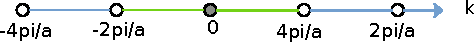
\includegraphics{figures/3_2_1D.pdf}
          \end{center}
          \begin{figure}[H]
              \centering
              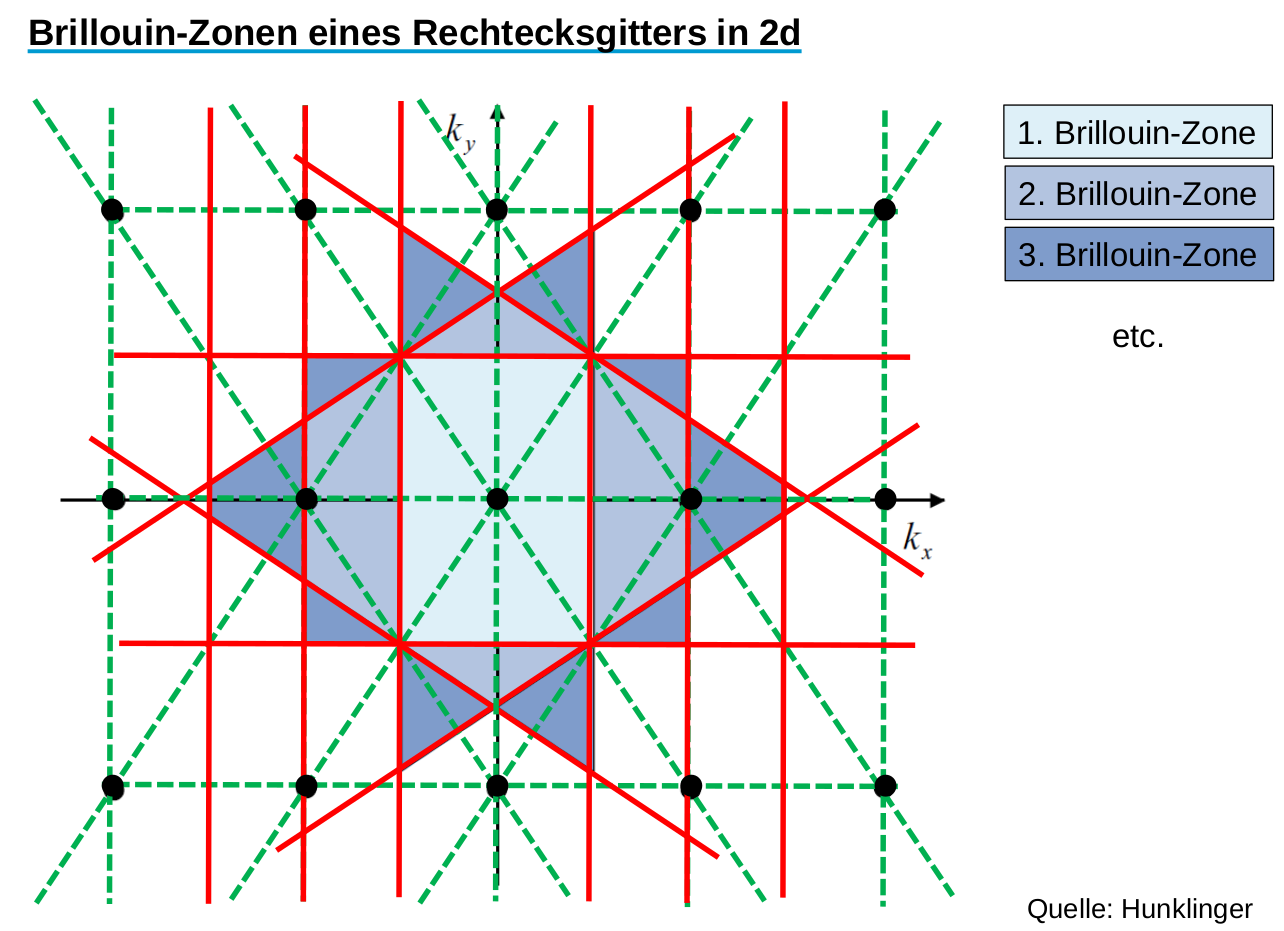
\includegraphics[width=0.6\textwidth]{figures/3_2_2D.png}
              \caption{Brillouin-Zonen 2D}
              \label{}
          \end{figure}
          Rechtecksgitter:
          \begin{itemize}
              \item[1. BZ:] Rechteck
              \item[2. BZ:] 4 Teilflächen, die sich durch Verschiebung um \textbf{rez. Gitterverktoren} zu Rechteck der 1. BZ Zusammensetzen lassen.
              \item[3. BZ:] (und höhere) Je höher die Ordnung der BZ, desto mehr/komplizierte Teilflächen. Durch Verschiebungum rez. GV $\Rightarrow$ Rückführung auf 1. BZ
          \end{itemize}
          \begin{figure}[H]
              \centering
              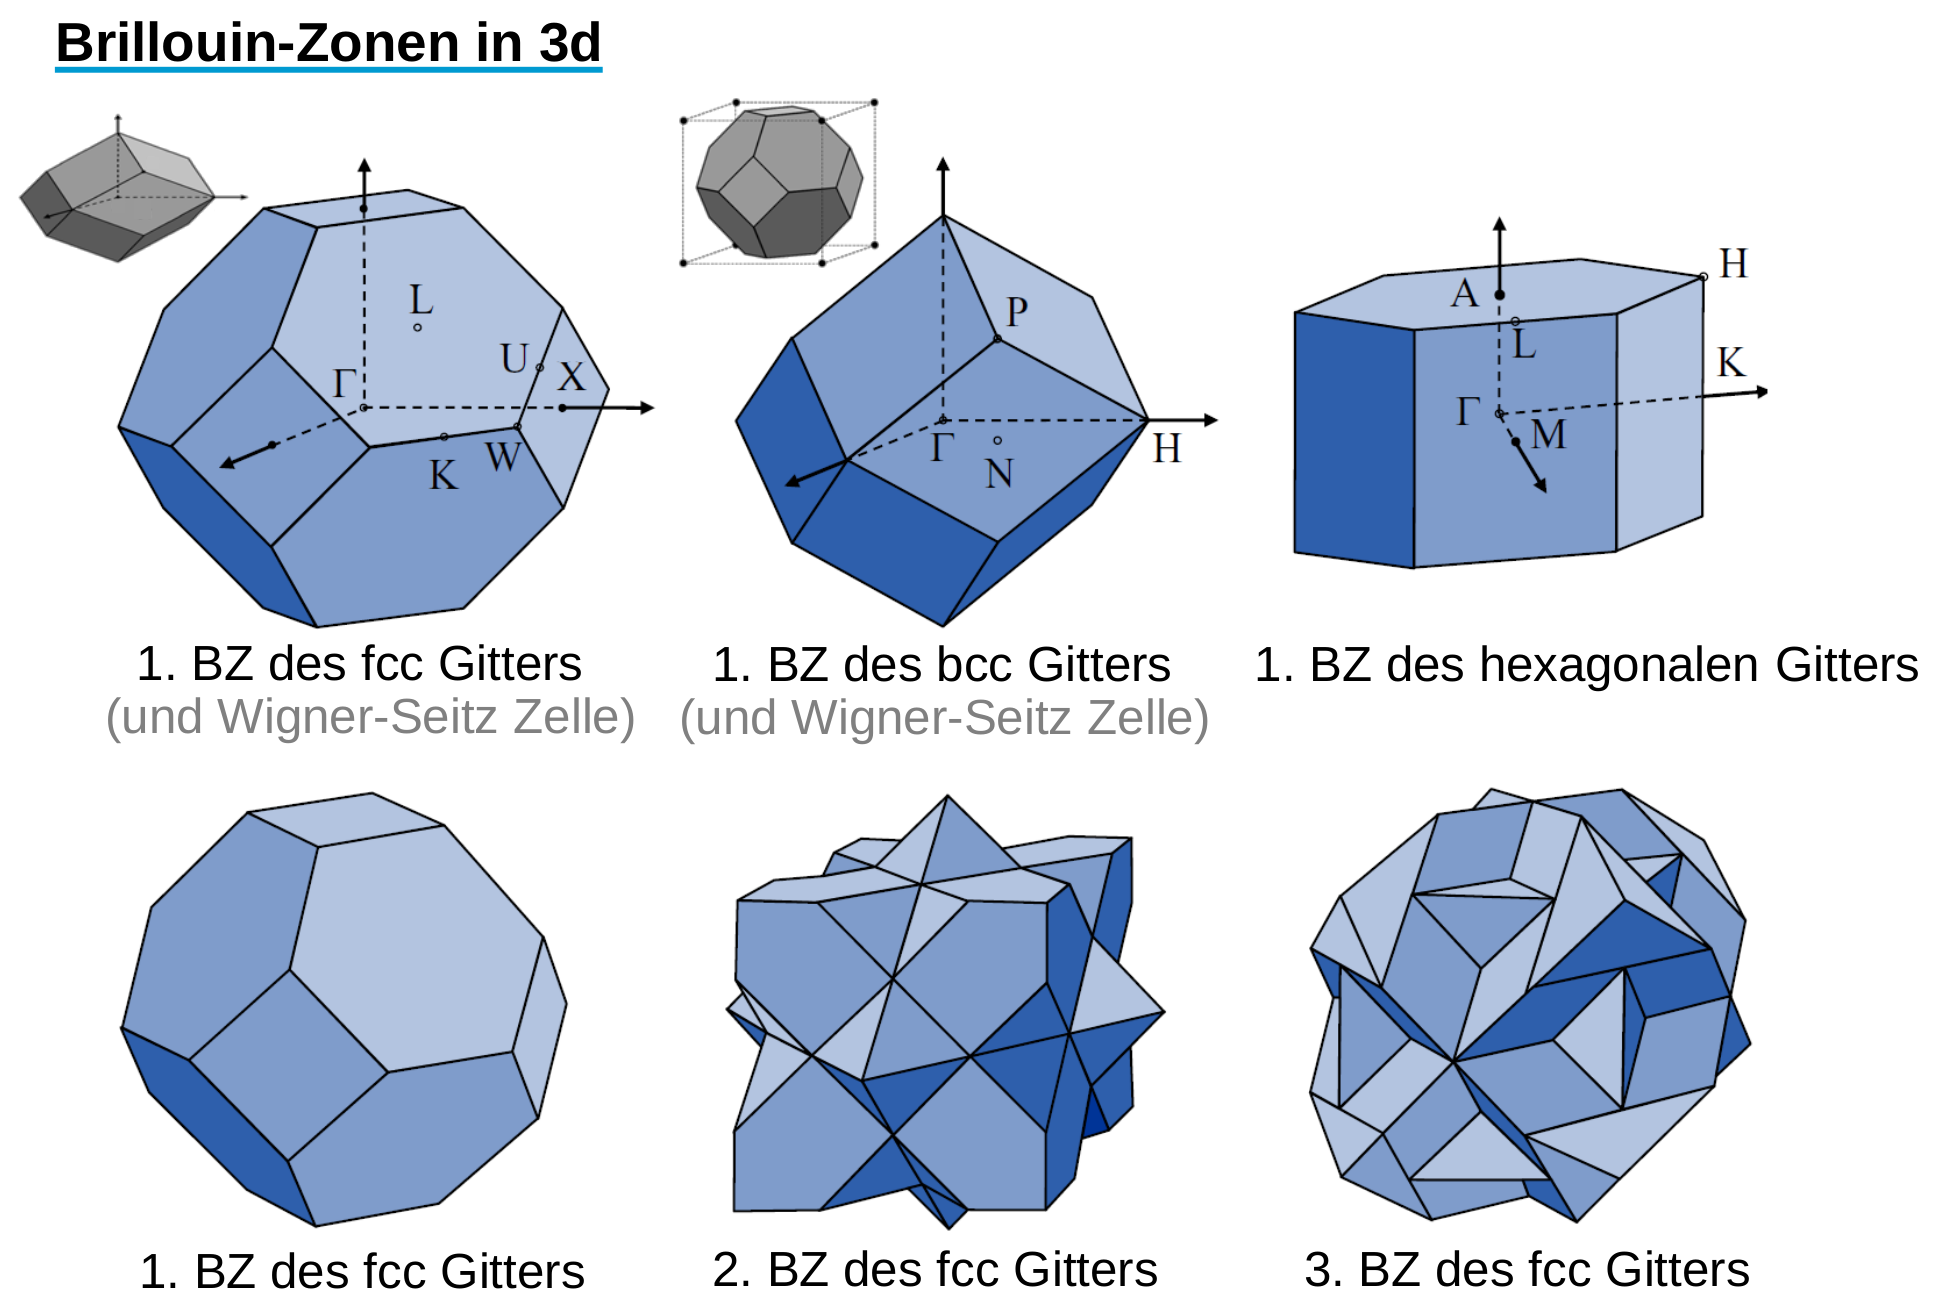
\includegraphics[width=0.6\textwidth]{figures/3_2_3D.png}
              \caption{Brillouin-Zonen 3D}
              \label{}
          \end{figure}
          Auch in 3D: BZ höherer Ordnung aus immer mehr Einzelteilen zusammengesetzt. Durch Verschiebung um rez. GV erhält man Polyeder, der in Größe und Gestalt der 1. BZ entspricht.\\
          \textbf{Diskussion:}
          \begin{itemize}
              \item 1. BZ ist Wigner-Seitz-Zelle des rez. Raums
              \item Durch periodischs Aneinanderreihen der 1. BZ lässt sich der reziproke Raum vollständig auffüllen.
              \item Punkt hoher Symmetrie werden Symbole ($\rightsquigarrow$ Gruppentheorie) zugeordnet, z.B. $\Gamma$-Punkt: Zentrum der 1. BZ, X-Punkt: Schnittpunkt der 1. BZ mit x.Achse
          \end{itemize}
    \item[(c)] \textbf{Miller-Indizes}
          Zwischen den Miller-Indizes zur Bezeichnung von Gitterelementen des realen Gitters und dem reziproken Gitter besteht ein direkter Zusammenhang:\\
          \begin{itemize}
              \item[1.] Der reziproke Gittervektor $\textbf{G}_{hkl}$ steht senkrecht auf den Netzebenen (hkl) im realen Raum.\\
                    Begründung:
                    \begin{align*}
                        \textbf{G}_{hkl} & = h \textbf{b}_1 + k \textbf{b}_2 + l \textbf{b}_3\\
                        & =\frac{2 \pi}{V_0}\left[h(\textbf{a}_2\times \textbf{a}_3) + k(\textbf{a}_3\times \textbf{a}_1) + l(\textbf{a}_1\times \textbf{a}_2)\right]
                    \end{align*}
                    vgl. Normalvektor auf $(hkl)$ \textbf{n}\\
                    $e^{i \textbf{G}_{nlk}\textbf{R}}$ und also hier $\textbf{n} e^{i \textbf{n} \textbf{R}} \overset{!}{=}1$ folgt $\textbf{n} \parallel \textbf{G}_{hkl}$.
              \item[2.] Der Abstand zweier benachbarter Netzebenen im realen Raum ist durch den Betrag des kürzesten reziproken Gittervektors $\left| \textbf{G}_{nlk}^{min} \right|$ bestimmt:
              $$d_{hkl} = \frac{2 \pi}{\left| \textbf{G}_{nlk}^{min} \right|} $$
              Begründung: Für $\left| \textbf{G}_{nlk}^{min} \right| = \frac{2 \pi}{d_{hkl}}$ ist $e^{i \textbf{G}_{nlk}^{min} \textbf{R}} = 1$ mit $\lambda = 2 \pi \left| \textbf{G}_{nlk}^{min} \right|^{-1} = d_{hkl}$
          \end{itemize}
\end{itemize}



\subsection{Streuung an Kristallen} \label{kap:3_3}
Streuintensität:
\begin{align*}
    I(\Delta \textbf{k}) \sim |A_B (\Delta \textbf{k})|^2 \sim \left| \int_{V} \rho(\textbf{r})e^{-i \Delta \textbf{k} \cdot \textbf{r}} \mathrm{d}^3r\right|^2 = \left|\mathcal{A}(\Delta\textbf{k})\right|^2 
\end{align*}
mit Streuvektron $\Delta \textbf{k} = \textbf{k}_2-\textbf{k}_1$
\begin{itemize}
    \item Vorfaktoren sind zunächst nicht von Bedeutung, da Abhängigkeit von $I$ con$\Delta \textbf{k}$ untersucht
    \item Vorsicht: In der Literatur werden manchmal $A_B$ und $\mathcal{A}$ als Streuamplitude bezeichnet.
\end{itemize}
Mit Kap. \ref{kap:3_2}:
\begin{align*}
    \left| \mathcal{A} ( \Delta \textbf{k}) \right| ^2 = \left| \sum_{hkl} \rho_{hkl} \int_V e^{i(\textbf{G} - \Delta \textbf{k})\textbf{r}} \mathrm{d}^3 r \right|^2
\end{align*}

\begin{itemize}
    \item[$\rightarrow$] Im allgemeinen Fall $\Delta \textbf{k} \neq \textbf{G}$:$e$-Funktion hat kompexe Exponenten und oszilliert. Bei großem V (d.h. größer als Oszillationsperiode $\left(1 /(\textbf{k}\cdot \textbf{G})\right)^3$) mitteln sich die Beträge weg.\\
    Physikalisch: Streubeiträge der einzelnen Atome interferieren destruktiv.
    \item[$\rightarrow$] Spezialfall $\Delta \textbf{k} = \textbf{G}$: e-Funktion hat den Wert 1.\\
    Physikalisch: Beiträge der einzelnen interferieren konstruktiv.
\end{itemize}

\begin{align*}
    \left| \mathcal{A} ( \Delta \textbf{k}) \right| ^2 = \begin{cases}
        0 & \text{für } \Delta \textbf{k} \neq \textbf{G}\\
        \left| \rho_hkl\right|^2 \cdot V^2 &  \text{für } \Delta \textbf{k} = \textbf{G}_{(hkl)}
    \end{cases}
\end{align*}
\begin{itemize}
    \item Streuung am Kristall: Streusignal $\neq 0$ nur, wenn Bedingung $\Delta \textbf{k} = \textbf{G}$ erfüllt. (Von Laue Bedingung)
    \item Bei realen Kristallen endliches V, endliche Eindringtiefe der Bedingung\dots
    \item Bei fester Lage der Probe (Kristalls) tritt in den meisten Richtungen keine Streuung auf. Bei Beugungsexperimente muß Kristallorientirung so lange gedreht werden, bis $\Delta \textbf{k} = \textbf{G}$, also ein Streusignal (Beugungsreflex) auftritt.
    \item Warum $\sim V^2$?\\
    $|\mathcal{A}(\Delta \textbf{k})|^2$ entspricht Intensität im Maximum des Beugungsreflexes Endliches V führt zu Verbreiterung $\sim V$\\
    Intergrierte Intensität des Beugungsreflexes $\sim \frac{V^2}{V} = V \sim$ Anzahl der Streuzentren.\\
    Auch Eindringtiefe trägt zu Verbreiterung bei. Z.B. Röntgenstrahlung: $10^{-5}-10^{-3}$ pro Netzebene.
\end{itemize}

\begin{itemize}
    \item[(a)] Ewald-Kugel und Bragg Bedingung\\
    \textbf{Ewald Konstruktion:}
    \begin{itemize}
        \item[(1)] Zeichne reziproke Gitter, wähle Gitterpunkt
        \item[(2)] Einzeichnen von einfallendem Wellenvektor als \textbf{-k} von diesem
        \item[(3)] Endpunkt von $-\vk$ (Anfang von \textbf{k}) sei Mittelpunkt der \textbf{Ewald-Kugel} (2D: Ewald-Kreis) mit Radius k.
        \item[(4)] Für rez. Gitterpunkte, die auf dieser Kugel liegen, ist von Laue Bedinugn $\dvk = \vk' - \vk \overset{!}{=} \textbf{G}$ erfüllt. Der gebeugte Strahl tritt dann mit Wellenvektro $\vk' = \vk + \textbf{G}$ aus. In dieser Richtung tritt Beugungsreflex auf.
        \item[(5)] Verschmierung der reziproken Gitterpunkte $\rightarrow$ endliches Probenvolumen.
    \end{itemize}
    \textbf{Diskussion:}\\
    Durch expt. Anordnung des Beugungsexperiments und ORientierung der Probe liegt $\dvk$ bzgl. des reziproke Gitters fest.\\
    $\rightarrow$ Beugungsreflex $\rightarrow \textbf{G}_{hkl} \rightarrow \rho_{hkl} \rightarrow \textbf{G}_{hkl} \bot (hkl)$\\
    d.h. Beugungsreflex resultiert aud Streuung an Netzebenenschar, also periodischen Streudichtevariation mit Periode $d_{hkl}$. Zusammenhang von Laue Bedingung und Bragg-Bedingugn Betrachte Steuung als Funktion des Winkel $\Theta$ zwsche $\vk$ und (hkl).
    \begin{figure}[H]
        \centering
        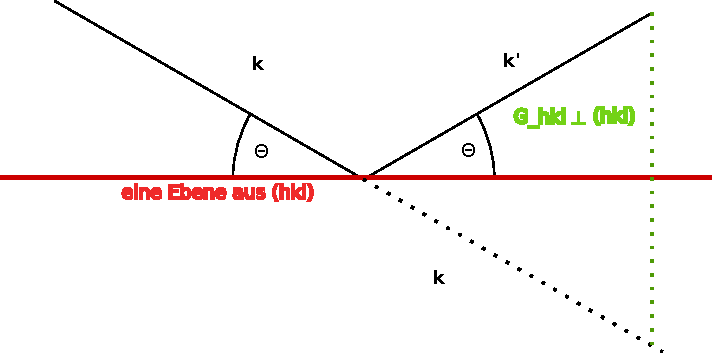
\includegraphics{figures/3_3Reflection.pdf}
        \caption{$|\textbf{G}_{hkl}|=2\cdot k \sin(\Theta) = \frac{4\pi}{\lambda}\sin(\Theta)$ mit $\lambda=\frac{2\pi}{k}$\\ }
        \label{fig:3_3Reflection}
    \end{figure}
    mit (2) 
    \begin{align*}
        \textbf{G}_{hkl} = n \textbf{G}_{hkl}^{min} n\frac{2\pi}{\textnormal{d}_{hkl}} = \frac{4\pi}{\lambda}\sin{\Theta} \Longleftrightarrow 2\cdot \textnormal{d}_{hkl}\sin{\Theta}= n \lambda
    \end{align*}
    \item[(b)] Strukturfaktor:\\
    Bisher nur Ort von Beugungsreflexen ($\Delta \textbf{k} = \textbf{G})$, für Intensitäten wird Fourier-Koeffizient
    \begin{align*}
        \rho_{hkl} = \frac{1}{V_0} \int_{V_0} \rho (\textbf{r}) e^{-i \textbf{G} \textbf{r}} \mathrm{d}^3r \quad \text{mit } V_0 \text{ primitive EZ}
    \end{align*}
    \begin{itemize}
        \item[$\rightarrow$] Information über Aufbau der Basis.\\
        Streubeiträge der Basisatome können konstruktiv o. destruktiv interferieren.
        \begin{itemize}
            \item[$\rightarrow$] Stärke des Beugungsreflexes
        \end{itemize}
    \end{itemize}
    Aufteilung der Streudichteverteilung af Basisatome:
    \begin{align*}
        \textbf{r} = \textbf{R}_n + \textbf{r}_\alpha + \textbf{r}'
    \end{align*}
    $\textbf{R}_n$: Ursprung EZ, $\textbf{r}_\alpha$: $\alpha$-tes Atom, $\textbf{r}'$: Ortsvektor von $\alpha$-tem Atom.\\
    mit:
    \begin{align*}
        \textbf{r}_\alpha = u_\alpha \textbf{a}_1 + v_\alpha \textbf{a}_2 + w_\alpha \textbf{a}_3
    \end{align*}
    \begin{itemize}
        \item[$\rightsquigarrow$] Für jede Art von streuender Welle und zugehöriger WW gerechtfertigt, weil die Streudichteverteilung immer noch um Atom konzentriert ist.
    \end{itemize}
    \begin{itemize}
        \item Röntgenbeugung: Schalenelektronen
        \item Neutronenbeugung: Kernen
    \end{itemize}
    \begin{align*}
        \Rightarrow \qquad \rho_{hkl} = \frac{1}{V_0} \sum_{\alpha} e^{-i \textbf{G} \textbf{r}_{\alpha}} \underbrace{\int_{V_{\alpha}} \rho_{\alpha} (\textbf{r}') e^{-i \textbf{G} \textbf{r}'} \mathrm{d}^3r'}_{=: f_{\alpha} (\textbf{G})\text{ Atom-Formfaktor ($\rightarrow c$)}}  = \frac{1}{V_0} \underbrace{\sum_{\alpha} e^{-i \textbf{G} \textbf{r}_{\alpha}} f_{\alpha} (\textbf{G})}_{=: S_{hkl}}
    \end{align*}
    $\text{Strukturfaktor:} \qquad S_{hkl} = \sum_{\alpha} e^{-i \textbf{G} \textbf{r}_{\alpha}} f_{\alpha} (\textbf{G})$
        \begin{itemize}
        \item[$\rightarrow$] Beschreibt Einfluss der Interferenz der Basisatome auf dei Streuverteilung.
        \begin{align*}
            S_{hkl} = \sum_\alpha f_\alpha e^{-2\pi i (hu_\alpha+kv_\alpha+lw_\alpha)}
        \end{align*}
        \item[$\rightarrow$] \textbf{Spezialälle:}
        \begin{itemize}
            \item[(i)] Primitives Gitter (nur 1 Atom im Ursprung) $S_{hkl}=f(\textbf{G})$
            \item[(ii)] CsCl Gitter\\ $\text{Kubisch primitiv mit 2-atomiger Basis} \qquad \textbf{r}_{Cs}= \left(\begin{array}{c} 0 \\ 0 \\ 0 \end{array}\right) \textbf{r}_{Cl} = \left(\begin{array}{c} 1/2 \\ 1/2 \\ 1/2 \end{array}\right)$ 
            \begin{align*}
                S_{hkl} = \begin{cases}
                    f_{Cs} & \text{für $h+k+l$ gerade}\\
                    f_{Cl} & \text{für $h+k+l$ ungerade}
                \end{cases}
            \end{align*}

            \item[(iii)] bcc Giter (einfache Basis): \textbf{r}$_1 = \left(\begin{array}{c} 0 \\ 0 \\ 0 \end{array}\right)$, \textbf{r}$_2 = \left(\begin{array}{c} 1/2 \\ 1/2 \\ 1/2 \end{array}\right)$
            \begin{align*}
                S_{hkl} = \begin{cases}
                    2f & \text{für $h+k+l$ gerade}\\
                    0 & \text{für $h+k+l$ ungerade}
                \end{cases}
            \end{align*}

            \item[\textbf{Diskussion}]
            Im bcc Gitter (und in anderen zentrierten Gittern) Kommte es zur systematischen Anslöschung von Beugungsreflexen.\\
            Ursache: Destruktive Interferenz der Netzebene durch das im Ursprung liegende Atom und das Zentrierte Atom.
            \item[\textbf{Beispiel}(100)] (Beugungsreflex)
                \begin{figure}[H]
                    \centering
                    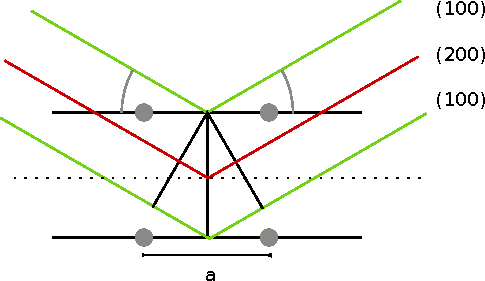
\includegraphics[]{figures/3_3Bragg.pdf}
                    \caption{}
                    \label{}
                \end{figure}
              % TODO
        \end{itemize}
    \end{itemize}
    \item[(c)] \textbf{Atomformfaktor}\\
    Streuvermögen eines einzelnen Atoms $f_\alpha(\Delta \textbf{k}) = \int_{V_\alpha}\rho_\alpha(r_\alpha)e^{-i\Delta \textbf{k} \textbf{r}'} d^3r'$ \\
    {\footnotesize mit $\Delta \textbf{k} = \textbf{G}$}\\
    $\rightarrow$ Art der Wechselwirkung zwischen Welle und Atom.
    \begin{itemize}
        \item[(i)] \textbf{Neutronenstreuung}\\
        Streuung am Kern, Punktförmig, $\Delta \textbf{k} \cdot \textbf{r} \ll 1$
        \begin{align*}
            f_{\alpha} (\Delta \textbf{k}) = \int_{v_{\alpha}} \rho_{\alpha} (\textbf{r}') \mathrm{d}^3r' = -b
        \end{align*}
        -: Konvention, gemessen wird $|b|^2$\\
        $b$: Streulänge
        \item[(ii)] \textbf{Röngensteruung}
        Streuung an Elektronenhühlle $\sim a \sim \lambda$
        Annahme: kugelsymmetrische Ladungsdichteverteilung:
        \begin{align}
            f_\alpha(\Delta \textbf{k}) &= 
            \int_{0}^{R_\alpha} \mathrm{d}r
            \int_{0}^{\pi} \mathrm{d}\theta
            \int_{0}^{2\pi} \mathrm{d}\phi \rho_\alpha(r) r^2 \sin(rl)e^{-i\Delta k r \cos{\theta}}\nonumber\\
            &= \int_{0}^{R_\alpha}4\pi r^2 \rho(r)\frac{\sin{\Delta k \cdot r}}{\Delta k \cdot r} \mathrm{d}r \label{eq:rstr}
        \end{align} 
        z.B. H-Atom:
        \begin{align*}
            \rho (r) = \left| \Psi_0 (r) \right|^2 = \left| \sqrt{\frac{1}{\pi a_0^3}} \cdot e^{-r/a_0} \right| ^2 = \frac{1}{\pi a_0^3} \cdot e^{-2r/a_0}
        \end{align*}
        in (\ref{eq:rstr}) und Limes $R_{\alpha} \rightarrow \infty$:
        \begin{align*}
            f_H (\Delta k) = \left[ \frac{1}{1+(\frac{1}{2} a_0 \Delta k)^2}\right]^2
        \end{align*}
        Vereinfachung für $\Delta k \cdot r \rightarrow 0$:
        \begin{align*}
            \lim_{\Delta k r \rightarrow 0}f_H(\Delta k) = \int_0^{R_\alpha}4\pi r^2 \rho(r)\dr = Z\\
            \rightarrow \qquad f_H = Z \quad \text{oder Streuintensität} \quad \sim Z^2
        \end{align*}
        Erfüllt für:\begin{itemize}
            \item Vorwärtsstreuung ($\Delta k = 0$)
            \item Näherungsweise punktförmige Atome ($R_\alpha \ll  a \approx \lambda$)
        \end{itemize}
    \end{itemize}
    \item[(d)] \textbf{Debye-Waller-Faktor}
    Berücksichtigt die thermische Fluktuation der Atome um ihre Gleichgewichtsposition.
\end{itemize}



\subsection{Experimentelle Methoden der Strukturanalyse durch Beugung} \label{kap:4_4}
\begin{itemize}
    \item[(a)] \textbf{Messverfahren}
    \begin{itemize}
        \item[(i)] \underline{Drehkristallverfahren:}\\
        Voraussetzung - Einkristall; - monochromatische Strahlung (festes $\lambda$)\\
        Messprinzip: Voraussetzung $\Delta \textbf{k} = \textbf{G}$ ist bei gegebenem $\Delta \textbf{k}$ in der Regel nicht erfüllt. Drehung des Kristalls um eine Achse. Für bestimmte Winkel ist Streubedingung für bestimmte Netzebenenschar erfüllt.\\
        Nach Möglichkeit Drehachse = Symmetische Achse de Kristalls, z.B. $\textbf{a}_3$
        \begin{itemize}
            \item[$\rightarrow$] Netzebenen $||$ Drehachse: \textbf{G}$_{nk0}$ (l=0)\\
            Streuung in xy Ebene, Reflexe falls $\Delta k$ = $G_{hk0}$
            \item[$\rightarrow$] Netzebenen $\nparallel$ Drehachse: $\textbf{G}_{hkl}$\\
            Streuung ausserhalb xy-Ebene, vertikale Verschiebung der Beugungsreflexe für $l = \pm 1, \pm 2, \dots$
            % \begin{figure}[H]
            %     \centering
            %     \includegraphics[]{}
            %     \caption{Typische Detektion mit zylindrischem Film.}
            % \end{figure}
	   \end{itemize}
	   \item[ii)] Debye-Scherrer-Verfahren (Pulvermethode):
		Kristallpulver (Kristallite mit zufällig orientierter Richtung), monochromatische Strahlung.\\
		\textbf{Messprinzip:}  Streubedingung $\Delta \textbf{k} = \textbf{G}$ lässt sich für festes \textbf{k} immer erfüllen (durch passend orientierte Kristallite)\\
		$\rightarrow$ Alle Beugungsreflexe zu festem \textbf{G} liegen auf einem Kegelmantel der konzentrisch zum einfallenden Strahl ausgerichtet ist und Öffnungswinkel $2\Theta$ besitzt.
		\begin{figure}[H]
			\centering
			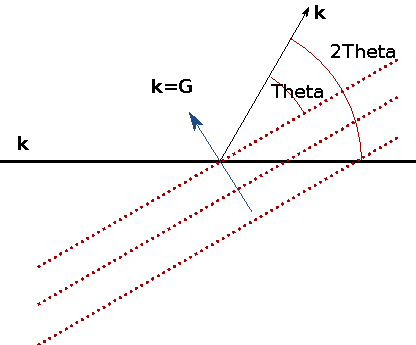
\includegraphics{figures/3_4RefKrist.pdf}
			\caption{Vorteile, sehr präzise, z.B. Bestimmung von Gitterkonstanten}
			\label{}
		\end{figure}
		\item[iii)] Laue-Verfahren:
		Einkristall, Kontinuumsstrahlung ('alle' $\lambda$) Messprinzip: $\Delta \textbf{k} = \textbf{G}_{hkl}$ wird durch den zu (hkl) passenden Wellenvektor \textbf{k} erfüllt ($|k| = \frac{2\pi}{\lambda}$) $\rightarrow$ Punktmuster aus Beugungsreflexen. \\
		$\rightarrow$ EInstrahlung längs Symmetrierichtung läuft Beugunsbild, welches die Symmetrie diese Achse widerspiegelt $\rightarrow$ Orientierung von Proben.
	\end{itemize}
	\item[(b)] \textbf{Praktische Aspekte}\\
	Allgemiener Aufbau:
	\begin{itemize}
		\item Quelle
		\item Monochromator (falls erforderlich)
		\item Probe
		\item Detektor
	\end{itemize}
	\begin{figure}[H]
		\centering
		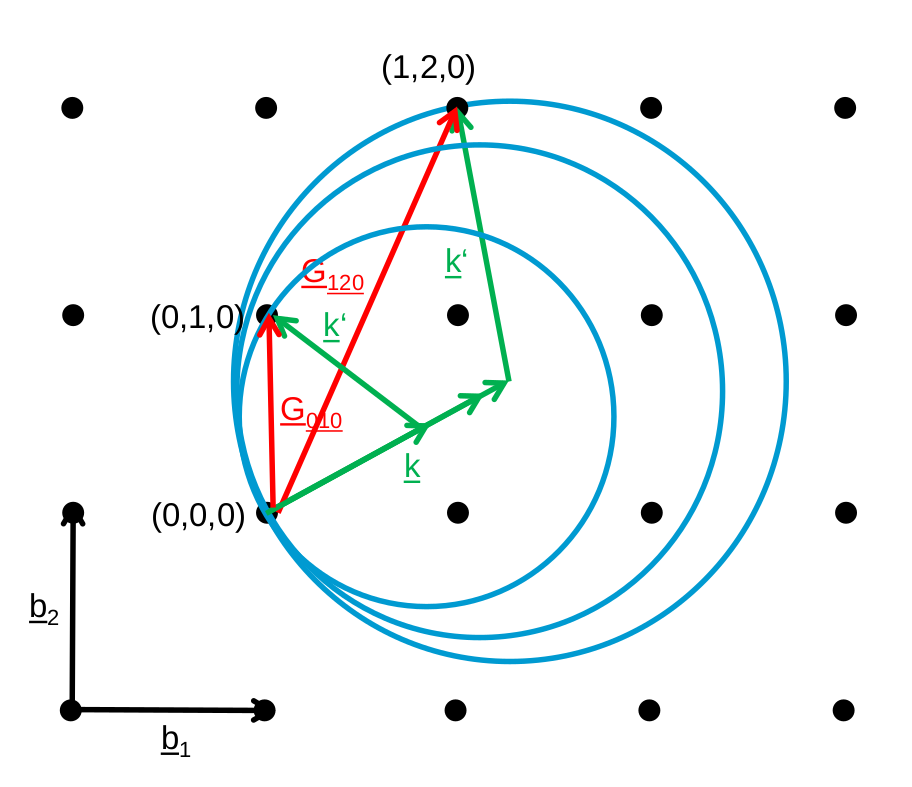
\includegraphics[width=0.7\textwidth]{figures/3_ewald.png}
		\caption{Ewald Konstruktion. Laue Verfahren (Vorlesungsfolie)}
		\label{}
	\end{figure}
\end{itemize}